%----------------------------------------------------------------------------------------
%	PACKAGES AND OTHER DOCUMENT CONFIGURATIONS
%----------------------------------------------------------------------------------------
\documentclass[a4paper, 12pt]{article}
 
\usepackage[T1]{fontenc}		                    % Selecao de codigos de fonte.
\usepackage[utf8]{inputenc}		                    % Codificacao do documento (conversão automática dos acentos)
\usepackage{indentfirst}		                    % Indenta o primeiro parágrafo de cada seção.
\setlength{\parindent}{1.0cm}                       % 1.0 cm de paragrafo
\usepackage{nomencl} 			                    % Lista de abreviaturas e siglas
\makenomenclature
\usepackage{color}	             			        % Controle das cores
\usepackage{graphicx}			                    % Inclusão de figuras
\usepackage{subfigure}                              % Inclusão de subfiguras
\usepackage{microtype} 		           	            % Para melhorias de justificação
\usepackage[brazil]{babel}                          % Linguagem do documento
\usepackage{amsmath, amsfonts, amssymb}             % Pacotes de funções extras de matemática
\usepackage[colorinlistoftodos]{todonotes} 
\usepackage[left = 3cm, right = 2cm, top = 3cm, bottom = 2cm, headsep = 0.5cm, footskip = 1cm]{geometry} 
%\usepackage[version=3]{mhchem}                  % Package for chemical equation typesetting. \ce{equation}
%\usepackage{siunitx}                            % Provides the \SI{}{} and \si{} command for typesetting SI units
\usepackage[font=small,labelfont=bf]{caption}   % Custom captions under/above floats in tables or figures
\usepackage{lettrine}                    % The lettrine is the first enlarged letter at the beginning of the text
\usepackage{titling}                     % Customizing the title section
\usepackage{blindtext}                   % Package to generate dummy text throughout this template 
\usepackage{float}                       % 
\usepackage{epigraph}                    % Colocar epígrafos
\usepackage{rotating}
\usepackage{natbib}
\setcitestyle{authordata, round, citesep={semicolon}, aysep={,}, yysep={&}}
%\usepackage[alf, abnt-and-type=e]{abntex2cite}
%\citeoption{abnt-etal-cite=3}
\usepackage{fancyhdr}                    % Modificar Cabeçalho e Rodapé
\usepackage{setspace}                    % espacamento entre linhas
\onehalfspacing                          % padrao 1.5 de espacamento entre linhas

\setstretch{1.5}

%----------------------------------------------------------------------------------------
%	Definir Qual Fonte de Texto Usar no Documento
%----------------------------------------------------------------------------------------
\usepackage{helvet}
\renewcommand{\familydefault}{\sfdefault}
%\usepackage{lmodern}			 % Usa a fonte Latin Modern
%\usepackage{Arial}              % Uncomment to use the Arial font 
%\usepackage{times}              % Uncomment to use the Times New Roman font
%\usepackage[sc]{mathpazo}       % Use the Palatino font
%----------------------------------------------------------------------------------------


%----------------------------------------------------------------------------------------
%	Hiperlinks
%----------------------------------------------------------------------------------------
\usepackage[breaklinks = true]{hyperref}   % Fazer um e-book
\usepackage{url}                           % Colocar links
\usepackage{xcolor}
\hypersetup{
    colorlinks,
    linkcolor={black},
    citecolor={black},
    urlcolor={black}
}
% Fazer sumir aquelas bordas zuadas nos hiperlinks, pode mudar as cores de tudo!
%----------------------------------------------------------------------------------------


%----------------------------------------------------------------------------------------
%	Modificar os titulos
%----------------------------------------------------------------------------------------

\usepackage{titlesec} % Allows customization of titles
\titleformat{\chapter}[block]{\LARGE\bfseries\centering}{\thechapter.}{0.5em}{} % Change the look of the section titles
\titlespacing{\chapter}{0pt}{*-4}{*2}
%\renewcommand\thesection{\Roman{section}} % Roman numerals for the sections
%\renewcommand\thesubsection{\roman{subsection}} % roman numerals for subsections
\titleformat{\section}[block]{\large\scshape\bfseries\flushleft}{\thesection.}{1em}{} % Change the look of the section titles
%\titleformat{\subsection}[block]{\large}{\thesubsection.}{1em}{} % Change the look of the subsection titles

%----------------------------------------------------------------------------------------

%----------------------------------------------------------------------------------------
%	TITLE SECTION
%----------------------------------------------------------------------------------------
\usepackage{fancyhdr} % Headers and footers

\fancypagestyle{formato}{
\lhead{\leftmark}
\chead{\empty}
\rhead{\empty}

\lfoot{\empty}
\cfoot{\thepage}
\rfoot{\empty}
}

\fancypagestyle{referencias}{
\lhead{REFERÊNCIAS}
\chead{\empty}
\rhead{\empty}

\lfoot{\empty}
\cfoot{\thepage}
\rfoot{\empty}
}

%----------------------------------------------------------------------------------------
%    Coisas que a Cano colocou que eu não entendo
%----------------------------------------------------------------------------------------
\newcommand{\R}{\mathbb{R}}
\newcommand{\N}{\mathbb{N}}
%\pagestyle{empty}
\def\linha#1{%
  \hbox to \hsize{%
      \vbox{\centering #1}}%
      \vspace{4mm}}

%----------------------------------------------------------------------------------------

\begin{document}
%----------------------------------------------------------------------------------------
%    Capa do TCC
%----------------------------------------------------------------------------------------


\begin{titlepage}
\thispagestyle{empty}
\begin{center}

\linha{{\large {UNIVERSIDADE FEDERAL DE SÃO PAULO}}}
\linha{{\large {INSTITUTO DE CIÊNCIA E TECNOLOGIA}}}
\linha{{\large {GRADUAÇÃO EM ENGENHARIA BIOMÉDICA}}}
\vspace{30mm}


\linha{\large NOME COMPLETO}
\vspace{30mm}

\linha{\bf \large TITULO DO TRABALHO}
\vspace{10mm}
\end{center}

\vfill

\linha{São José dos Campos, SP}
\linha{\large 2019}

\end{titlepage}

\begin{titlepage}
\thispagestyle{empty}
\begin{center}

\linha{{\large {UNIVERSIDADE FEDERAL DE SÃO PAULO}}}
\linha{{\large {INSTITUTO DE CIÊNCIA E TECNOLOGIA}}}
\linha{{\large {GRADUAÇÃO EM ENGENHARIA BIOMÉDICA}}}
\vspace{50mm}

\linha{\bf \large TITULO DO TRABALHO}

\vspace{25mm}
\end{center}

\begin{flushright}
\begin{minipage}{.60\linewidth} 
\textbf{Aluno:} NOME COMPLETO \\  
\textbf{Orientador:} NOME COMPLETO DO ORIENTADOR\\
\end{minipage}

\begin{minipage}{.60\linewidth} 
\vspace{8mm}
Trabalho de Conclusão de Curso apresentado ao Instituto de Ciência e Tecnologia da Universidade Federal de São Paulo como requisito parcial para obtenção do título de Graduação em Engenharia Biomédica.

\vspace{0.5 cm}
\end{minipage}

\end{flushright}

\vfill

\linha{São José dos Campos, SP}
\linha{\large 2019}
\end{titlepage}

\onehalfspacing

\begin{titlepage}
\linha{\large NOME COMPLETO}
\vspace{20mm}

\linha{\bf \large TITULO DO TRABALHO}

\vspace{15mm}

\begin{flushright}

\begin{minipage}{.50\linewidth}          
            
Trabalho de Conclusão de Curso apresentado ao Instituto de Ciência e Tecnologia da Universidade Federal de São Paulo como requisito parcial para obtenção do título de Graduação em Engenharia Biomédica.

\vspace{0.5 cm}
\end{minipage}

\end{flushright}

\vspace{15mm}
\begin{flushleft}
\begin{minipage}{.50\linewidth}  
Aprovado em: \line(40,0){22}/\line(40,0){22}/\line(40,0){22}\\
 \end{minipage}
\end{flushleft}
\vspace{5mm}

\begin{center}
\line(40,0){300}\\
NOME COMPLETO DO ORIENTADOR - Universidade Federal de São Paulo\\

\vspace{10mm}
\line(40,0){300}\\
BANCA 1 - Universidade Federal de São Paulo\\

\vspace{10mm}
\line(40,0){300}\\
BANCA 2 - Universidade Federal de São Paulo
\end{center}

\vfill


\linha{São José dos Campos, SP}
\linha{\large 2019}
\end{titlepage}
% \newpage
% \setcounter{page}{2}
% \thispagestyle{empty}
% \vspace*{\fill}
\thispagestyle{empty}
\epigraph{Eu não tenho sonhos, eu tenho objetivos.}{Harvey Specter}
\epigraph{Se você não é nada sem o traje, então não deveria usá-lo.}{Tony Stark}

\newpage
\thispagestyle{empty}
\begin{center}
\section*{AGRADECIMENTOS}
\end{center}

\onehalfspacing

Espaço para agradecimentos e dedicatórias.

\newpage
\thispagestyle{empty}
\begin{center}
\section*{RESUMO}
\end{center}

\blindtext

\textbf{Palavras-chave: }
\newpage
\thispagestyle{empty}

\begin{center}
\section*{ABSTRACT}
\end{center}

\blindtext

\textit{\textbf{Keywords:} }


\newpage
\pagestyle{empty}
\begin{center}
\renewcommand\listfigurename{LISTA DE FIGURAS}
\listoffigures
\end{center}

\newpage
\begin{center}
\renewcommand\listtablename{LISTA DE TABELAS}
\listoftables
\end{center}

\newpage
\begin{center}
\renewcommand{\nomname}{LISTA DE ABREVIAÇÕES}
\printnomenclature
%\textcolor{red}{Digitar isso no terminal: \\ makeindex TCC.nlo -s nomencl.ist -o TCC.nls}
\end{center}

\newpage
\begin{center}
\renewcommand\contentsname{SUMÁRIO}
\tableofcontents
\end{center}
\clearpage
\pagestyle{formato}
\pagebreak

\pagenumbering{arabic}
\setcounter{page}{12}

\section{INTRODUÇÃO}

\Blindtext

\newpage
\section{FUNDAMENTAÇÃO TEÓRICA}

\blindtext[5]

\subsection{subseção 1}

\Blindtext \cite{Haacke:1999, Landini:2005, Lauterbur:1973, Polli:2010}

\subsubsection{subsubseção 1}

\Blindtext \cite{Bloch:1946, Graaf:2001}.

\subsection{subseção 2}

\blindtext[5]

\subsubsection{subsubseção 2}

\blindtext[5]

\newpage
\section{OBJETIVO}

\blindtext \cite{Atkins:2012, Gonzalez:2007}

\newpage
\section{METODOLOGIA}

\blindtext

Imagens de ressonância magnética de um paciente que teve episódios de \textit{Status Epilepticus} (SE)\nomenclature{\textbf{SE}}{\textit{status epilepticus}} são mostrados na Figura \ref{Fig:hipocampos}

\begin{figure}[H]
\centering
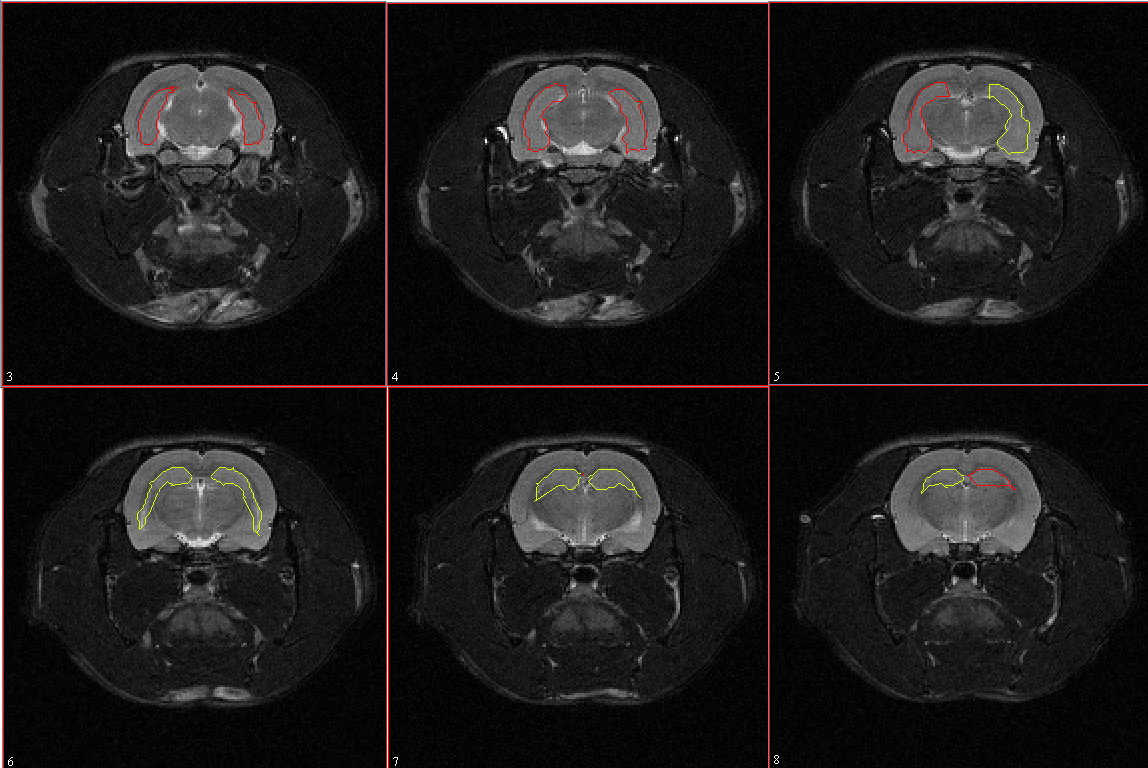
\includegraphics[scale=0.5]{Hipocampos.PNG}
\caption{Cortes coronais evidenciando os hipocampos. Fonte: Autor.}
\label{Fig:hipocampos}
\end{figure}	

\Blindtext

\pagebreak

\newpage

\section{RESULTADOS E DISCUSSÕES}
\label{Sec:Res_Dis}

\Blindtext

\pagebreak
\newpage
\section{CONCLUSÃO}

\blindtext

\pagebreak

\singlespacing
\addcontentsline{toc}{section}{REFERÊNCIAS}
\bibliographystyle{plainnat} % inserir referencias bibliograficas
\pagestyle{referencias}
\nocite{Prince:2014, Purcell:1946, Theodoridis:2009}
\bibliography{Ref_TCC}


%\newpage
%\addcontentsline{toc}{section}{ANEXO I}
%\section*{ANEXO I}


\end{document}
